\chapter{绪论}
\section{课题来源与意义}
近年来,随着 互联网(Internet)的兴起,互联网上的数据急剧膨胀。根据国际数据信息公司\footnote{https://www.idc.com/}(International Data Corporation, IDC)的统计和预测,2017 年全球网络数据量已经达到1.8ZB,到2025 年,全球数据总量预计还将增长50 倍。随着大量无标注数据的出现,也让研究人员开始考虑,如何利用现有的算法从这些大规模无标注的文本数据中自动挖掘规律和知识,以提取出有用的信息。自从2006年,加拿大多伦多大学教授 Geoffrey Hinton 提出的深度学习(Deep Learning, DL)概念以来\upcite{hinton2006reducing},为解决如何利用爆炸的数据量,以提取有效知识带来了新的思路。在这之后的发展中,基于神经网络的表示学习技术(Representation Learning)开始在各个研究领域崭露头角。尤其在图像(Image Classification)和语音自动识别(Automatic Speech Recognition,ASR)领域的多个任务上,基于表示学习的方法在性能上均超过了传统基于特征提取(Feature Extraction)的方法。

近年来,深度学习技术(Deep Learning)逐渐在自然语言处理中(Natural Language Processing, NLP)得到广泛应用。 例如,蒙特利尔大学教授 Yousha Bengio 提出用神经网络(Neural Network, NN) 来训练语言模型(Language Model)并进行了相关探索\upcite{DBLP:conf/nips/BengioDV00}。 后续的工作中,基于循环神经网络(Recurrent Neural Network, RNN)的语言模型建模方法由其学生 Tomas Mikolov 进行了极大拓展和完善\upcite{DBLP:conf/interspeech/MikolovKBCK10}。 网络通过学习能够将当前词的历史信息存储起来,以词的整个上下文(Context)作为依据,来预测下一个词出现的概率,克服了 N-gram 语言模型无法利用语句中长距离上下文依赖(Long Term Dependency)的缺点。 另外,在模型训练的过程中,由于词的历史信息被映射到低维连续空间,语义相似的单词被聚类,在语料中出现次数较少的词仍然能够得到很好的训练,不再需要额外的数据平滑技术(Smoothing Technology)。
迄今为止,采用RNN 训练的语言模型在模型困惑度(Perplexity, PPL)和识别系统的识别率(Accuracy)上都取得了最好的效果。

RNN 建模方法虽然表现出极大的优越性,但却是以牺牲计算复杂度为代价。 若训练大规模的文本语料,则需要花费很长的时间,制约了RNN 语言模型训练效率并且无法广泛应用到现实场景中去。 为克服这一不足,文献~\cite{DBLP:conf/icassp/MikolovKBCK11}~提出了多种优化策略来降低网络的计算复杂度,如缩短模型训练周期、减少训练数据集的规模、降低训练词表(Vocabulary)的大小、减少隐含层的节点数等,这些方法都在一定程度上降低了网络的运算量,提高了模型的训练效率,但同时也牺牲了较多的模型性能和精确度。 另外,在网络结构层面上,文献~\cite{DBLP:journals/coling/BrownPdLM92}~研究了一种基于分类的循环神经网络(Class-based RNN) 结构,网络的输出层被分解为两部分,增加的一部分称为分类层,从结构上降低了整个网络的计算复杂度,使得模型训练效率有了一定的提升且模型性能没有大的变化。 然而,在大词汇量连续语音识别系统中,采用此结构训练大规模语料语言模型仍需要花费大量时间。 因此,模型训练效率有待进一步优化。

\section{国内外研究现状}
语言模型可以用来对一段文本的概率进行估计,对信息检索(Information Retrieval)、机器翻译(Machine Translation)、语音识别(Speech Recognition)等任务有着重要的作用。语言模型的发展历史可以主要分为两个阶段:统计语言模型(Statistical Language Model)和神经网络语言模型(Neural Language Model)。其中统计模型主要指的是N-gram 语言模型,而随着深度学习的发展,神经网络语言模型产生了各种变体。我们接下来会一一介绍。

\subsection{N-gram 语言模型}
首先我们开始介绍传统的N-gram语言模型,它的意义不仅是提供了一种文本建模策略,而且定义了如何评价语言模型的好坏和相关拓展的问题。

形式化讲,统计语言模型的作用是为一个长度为$m$ 的字符串确定一个概率分布$p(w_1,w_2,\cdots,w_m)$,表示其存在或者出现的可能性,其中$w_1$ 到$w_m$ 依次表示这段文
本中的各个单词。一般在实际求解过程中,通常采用链式法则(Chain Rules)将计算序列概率分解成计算其条件概率值:
\begin{equation}
\label{equ:lm}
\begin{split}
p(w_1,\cdots,w_m) &= p(w_1) p(w_2|w_1) p(w_3|w_1,w_2)\cdots p(w_m | w_1,w_2,\cdots,w_{m-1}) \\
=&p(w_1)\prod_{t=1}^{m}p(w_t|w_1,\cdots,w_{t-1})
\end{split}
\end{equation}
在实际求解过程中,如果文本的长度较长,公式~\ref{equ:lm}~右部$ p(w_m | w_1,w_2,\cdots,w_{m-1}) $ 的估算会非常困难并且不准确。因此,研究者们提出使用一个简化模型:n 元模型(n-gram model)。在n 元模型中估算条件概率时,距离大于等于n 的上文词会被忽略,也就是对上述条件概率做了以下近似:
\begin{equation}
\label{equ:approx}
p(w_i | w_1,w_2,\cdots,w_{t-1})  \approx p(w_i | w_{t-(n-1)},\cdots,w_{t-1})
\end{equation}
当$n = 1$ 时,该模型称为称一元模型(unigram model),公式.~\ref{equ:approx} 右部会退化成$p(w_i)$,此时,整个句子的概率计算公式为:$p(w_1,w_2,\cdots,w_m) = p(w_1)p(w_2) \cdots p(w_m)$。从式中可以知道,一元语言模型中,文本的概率为其中各单词出现的概率的乘积。也就是说,模型假设了各个单词之间都是相互独立的,文本中的单词的先后顺序信息完全丢失。因此,该模型虽然估算方便,但性能有限而且实际精确度并不高。当$n = 2$ 时又称二元模型(bigram model),代入公式.~\ref{equ:approx}~中,右部为 $p(w_t|w_{t-1})$。常用的还有 $n = 3$ 时的三元模型(trigram model),使用$p(w_t |w_{t-2},w_{t-1})$ 作为近似。这些方法均可以保留一定的词序信息。

传统方法采用单词或者n元组的词频来作为n元组的概率计算方法,该方法简单有效能满足线上负载的计算需求。但是随着n的增大,模型的参数呈现指数爆炸式增长、概率计算复杂度也相应上升。目前谷歌有在线存储的最大的9元模型(Google Ngram Viewer)\footnote{https://books.google.com/ngrams},这已经是目前计算机系统存储,数据访问的极限了。


神经网络的建模思路建立在ngram模型之上,主要解决的是如何对文本的上下文信息利用先用的模型进行建模。历史上的模型,我们可以主要划分为:: 传统前向传递神经网络(Feed Forward Neural Network, FFNN)、循环神经网络(Recurrent Neural Network, RNN)建模方案。 以下我们将一一探讨。


\subsection{前馈神经网络语言模型}
由于神经网络对参数进行高度共享,因此对低频词具有天然的平滑能力。这里所指的神经网络语言模型(Neural Probabilistic Language Model, NPLM) ,最早由Bengio等人在2001年提出\upcite{DBLP:conf/nips/BengioDV00}, 近年来一些学者开始展开这方面的研究,并取得一系列成果,如~\cite{DBLP:conf/acl/BaroniDK14,DBLP:journals/sigkdd/BellK07,DBLP:journals/pami/BengioCV13,DBLP:journals/tnn/BengioSF94}~。 但总体而言, 对NPLM的研究还处在起步阶段。具体而言,NPLM通过一个多层感知网络(Multi-Layer Perceptron, MLP)来计算公式.~\ref{equ:approx} 中概率。
\begin{figure}
  \centering
  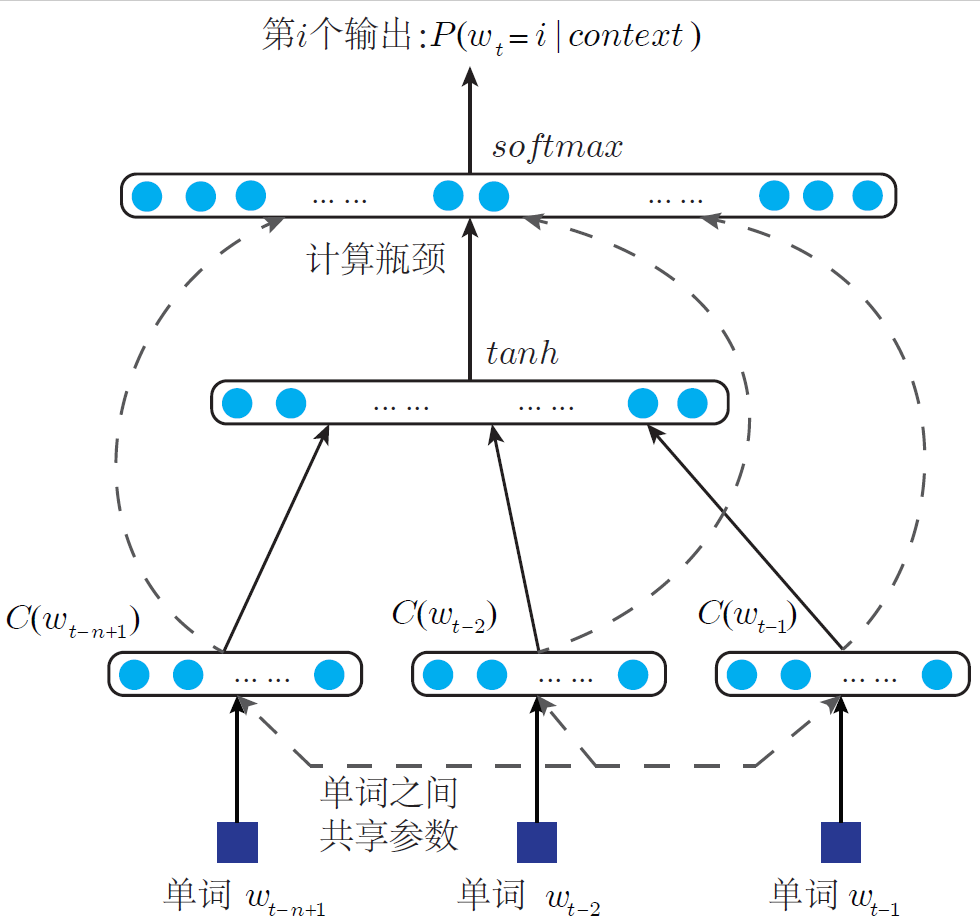
\includegraphics[width=0.6\linewidth]{./figures/nplm2.png}
  \caption{前馈神经网络语言模型。}\label{fig:nplm}
\end{figure}

图~\ref{fig:nplm} 给出一个典型的 NPLM 语言模型,神经网络语言模型采用普通的三层前馈神经网络结构。其中第一层为输入层,输入的是前$n$个单词;第二层是隐藏层,表征单词的上下文信息,最后一层是输出预测层,预测下一时刻的可能出现的单词概率分布。Bengio 提出使用各词的词向量作为输入以解决数据稀疏问题,因此输入层为词$w_{i-(n-1)}, \cdots,w_{i-1} $ 的词向量的顺序拼接:
\begin{equation}\label{equ:we}
  x = [e(w_{i-(n-1)}), \cdots , e(w_{i-2}), e{(w_{i-1})}]
\end{equation}
当输入层完成对上文的表示$x$ 之后,模型将其送入剩下两层神经网络,依次得到隐藏层$h$ 和输出层$y$:
\begin{equation}\label{equ:nplm}
\begin{split}
h =& \tanh(Hx+b) \\
y =&Wx + Uh +b'
\end{split}
\end{equation}
其中 $H \in \mathbb{R}^{|h| \times (n-1)|e|}$ 为输入层到隐藏层的权重矩阵,$U \in \mathbb{R}^{|\mathrm{V}|\times (n-1)|h|}$ 为隐藏层到输出层的权重矩阵,$ |\mathrm{V}|$表示词表的大小,$|e|$ 表示词向量的维度,$|h|$ 为隐藏层的维度。$b,b'$ 均为模型中的偏置项。矩阵$W \in \mathbb{R}^{|\mathcal{V}|\times (n-1)|e|}$ 表示从输入层到输出层的直连边权重矩阵。由于直连边 $W$ 的存在,该模型可能会从非线性的神经网络退化成为线性分类器。因此,Bengio 等人在文中指出,如果使用该直连边,可以减少一半的迭代次数;但如果没有直连边,可以生成性能更好的语言模型。因此在后续工作中,很少有使用输入层到输出层直连边的工作,下文也直接忽略这一项。如果不考虑$W$ 矩阵,整个模型计算量最大的操作,就是从隐藏层到输出层的矩阵运算$Uh$,后续的模型均有对这一操作的优化。

\subsection{对数双线性语言模型}
2007 年,Mnih 和Hinton 在神经网络语言模型(NNLM)的基础上提出了对数双线性语言模型(Log-Bilinear Language Model, LBL)~\upcite{DBLP:conf/icml/MnihH07}。LBL 与NNLM 的区别正如它们的名字所示,LBL 的模型结构是一个对数双线性结构;而NNLM的模型结构为前馈神经网络结构。具体来讲,LBL 模型的代价函数为:
\begin{equation}
\label{equ:lbl}
\begin{split}
   &\hat r=\sum_{i=1}^{n-1}{U_i e({w_i})}, \\
   &p(w_n=w|w_{1:n-1})=\frac{\exp(\hat r^\top e(w))}{\sum_j{\exp(\hat r^\top e(w_j))}}
\end{split}
\end{equation}
其中 $\hat r$ 代表了上下文信息,$U_i$ 是对应单词的权重向量。然后基于预测表示 $\hat r$ 和词汇表中所有单词 $e(w),w\in \mathcal{V}$ 的表示之间的相似度来计算下一个单词的分布。

LBL 模型的代价函数(公式~\ref{equ:lbl}) 与NNLM 的代价函数(公式~\ref{equ:nplm})主要有两个区别。1) LBL 模型中,没有非线性的激活函数$\tanh$,而由于NNLM 是非线性的神经网络结构,激活函数必不可少;2) LBL 模型中,只有一份词向量$e$,也就是说,无论一个词是作为上下文,还是作为目标词,使用的是同一份词向量。其中第二点(只有一份词向量),只在原版的LBL 模型中存在,后续的改进工作均不包含这一特点。

后来的几年中,Mnih 等人在LBL 模型的基础上做了一系列改进工作。其中最重要的模型有两个:层次对数双线性语言模型(Hierarchical LBL,HLBL)~\upcite{DBLP:conf/icml/MnihT12} 和基于向量的逆语言模型(inverse vector LBL,ivLBL)~\upcite{DBLP:conf/nips/MnihK13}。

\subsection{循环神经网络语言模型}
对于循环神经网络语言模型(RNNLM)来说,它则直接对$p(w_t | w_1,w_2,\cdots,w_{t-1}) $ 进行建模,而不使用公式~\ref{equ:approx}~对其进行简化~\upcite{mikolov2012statistical,DBLP:conf/interspeech/MikolovKBCK10} 。因此,RNNLM 可以利用所有的上文信息,预测下一个词,其模型结构如图~\ref{fig:rnnlm}~所示。
RNNLM 的核心在于其隐藏层的计算公式:
\begin{equation}
\label{equ:rnn}
  h_t \leftarrow  \phi(e(w_t) + U h_{t-1} +b),
\end{equation}
其中 $\phi$ 为非线性激活函数。与NPLM 不同,RNNLM 并不采用 n 元近似,而是使用迭代的方式直接对所有上文进行建模。在上述公式中,$h_t$ 表示文本中第 $t$ 个词 $w_t$ 所对应的隐藏层,该隐藏层由当前词的词向量 $e(w_t)$ 以及上一个词对应的隐藏层 $h_{t -1}$ 结合得到。

\begin{figure}
  \centering
  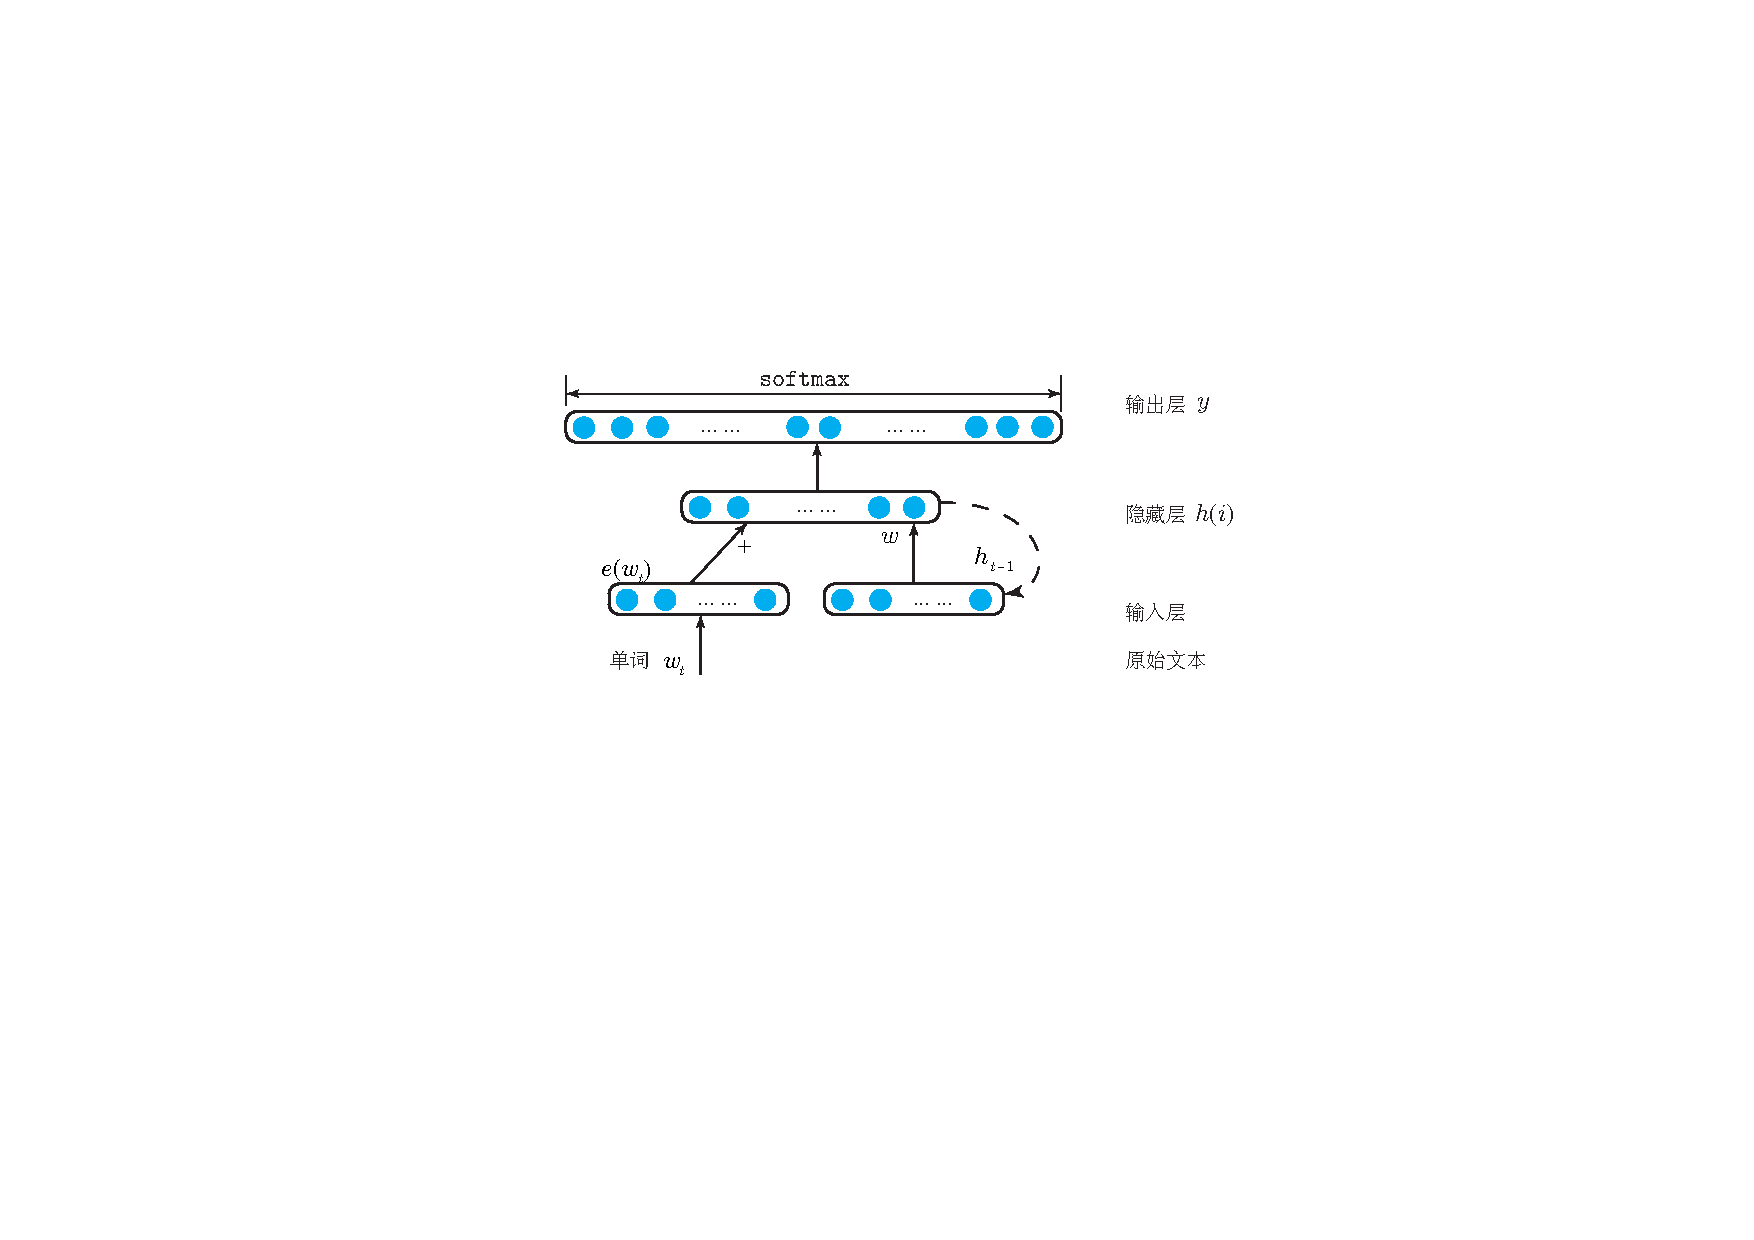
\includegraphics[width=0.68\linewidth]{./figures/rnnlm.pdf}
  \caption{循环神经网络语言模型结构图}\label{fig:rnnlm}
\end{figure}

隐藏层的初始状态为$h_0$,随着模型逐个读入语料中的词$w_1,w_2,\cdots$, 隐藏层不断地更新为$h_1,h_2,\cdots$ 。根据公式~\ref{equ:rnn}~,每一个隐藏层包含了当前词的信息以及上一个隐藏层的信息。通过这种迭代更新的方式,每个隐藏层实际上包含了此前所有上文的信息,相比NPLM 只能采用上文 n 元短语作为近似,RNNLM 包含了更丰富、更长的上文信息,也有更大的潜力达到更好的效果。最后,RNNLM 模型的输出层计算方法与NPLM 的输出层一致。


除了介绍的两种经典上下建模方法,最近研究提出来可以使用带有门限机制(Gating)的RNN来防止模型的长距离依赖问题,例如长短记忆网络(Long Short-Term Memory, LSTM), 门限记忆节点(Gated Recurrent Unit, GRU)和其他网络。


\section{论文研究内容}
在历史文献当中,源词和目标词分别被称为模型的输入和输出。源词通常可以用分布式表示(Distributed Representation)来表示,称为输入词嵌入(Word Embedding),可以使用基于外部语料库的连续词袋模型(CBoW)或Skipgram模型来训练。而这两个模型来源于语言模型任务,并且为了在特征空间中产生可能的嵌入分布而被大大简化。另外,输出字通常表示为字索引(Indexing)或~$1-K$~编码,并且可以与softmax概率函数直接关联。

语言模型的大词表问题是目前理论应用到实际过程中必须要克服的问题,我们当然可以通过配置高性能服务器来暂时延缓该问题的后果。但是一旦应用到大数据集上,即使是目前最好的中央处理器(CPU)或者图形处理器通用计算(GPU),仍然需要一个多月时间才能训练完善。因此,在保证原有模型的准确率和精度的前提下,如何提高模型的训练速度是我们主要讨论和研究的内容。为此我们讨论了两个不同的内容:上下文信息建模效率和精度对比和大词表问题的优化和研究。

针对上下文信息建模手段,目前主要采用的方案有以下几种:

一种是采用子词(Subword)或者字符级别的词(Character-level)来直接缩小词表大小;一种是通过采样技术(Sampling-based Approximation)来减少必要的训练时间;一种是通过基于分类的多元分类(class-based hierarchical softmax, cHSM)来加速模型和采用基于树模型的多层二元分类模型(tree-based hierarchical softmax, tHSM)。

同时,我们还需要针对CPU 和GPU设备分别进行探讨。因为传统的线性运算模型在流行的GPU并行运算方案中并不适用,所欲需要结合不同的运算设备分别讨论可行的方案。

在本节中,我们将这个目标词表示扩展到一个分层的形式,使它们适配基于类和基于树的分层概率计算。首先,我们提出了一个在分层结构上建模参数的字编码方案。因此,考虑到GPU上的并行吞吐性能,我们推导出紧凑的代价函数及其梯度。同时,类或树上的单词分布对其性能有很大的影响,应该在训练阶段之前定义,这些动态交换算法在训练过程中改变了单词群或子树结构在这个研究中。我们采用了几个分层聚类和词汇分割策略,用统计,句法和语义知识来初始化其结构,以达到一个稳定和可以预期的性能。而且,在推理过程中,不同于传统的softmax情况,得到最好的候选者自然是可行的,层次推理不能直接用 softmax 方法来实现。我们讨论基于树和基于类的搜索策略的两种不同的推理情况:a)打分:输出给定序列的概率;b)排序   :在给定的上下文中获取得分最高的一个候选单词。
\section{论文的组织结构}
\textbf{第一章:}``绪论'',主要介绍了本论文的研究背景和意义,另外简要说明了语言模型的发展历史以及本文的主要工作,并对本文的组织架构进行了说明。

\textbf{第二章:}``相关技术介绍'',

\textbf{第三章:}``并行树状概率模型'',


\textbf{第四章:}``并行层次概率模型'',

\textbf{第五章:}``语言模型实验及实验结果分析''

最后结论部分,总结了全论文的贡献和工作,并提出了未来的工作方向,同时撰写了结束语。



